\pagebreak
\section{Model Component}

The application needs a model to represent recipes. The recipe data we receive from the server is in JSON format, the data is then parsed to our application model. The model component is shown in \autoref{fig:model}.

\begin{figure}[H]
\centering
\includegraphics[width=0.67\linewidth, page=2]{img/model.pdf}
\caption{Application model}
\label{fig:model}
\end{figure}

We have two different representation of a recipe, \lstinline|Recipe| and \lstinline|IntermediateRecipe|. The \lstinline|IntermediateRecipe| is a small subset of a recipe which is used to display search results. When the user clicks the search results, then the rest of a \lstinline|Recipe| is downloaded from the server and displayed to the user.

A \lstinline|Recipe| consists of one or more instruction steps and one or more \lstinline|IngredientGroup|s which is a grouping of ingredients. The use of ingredients are easier understood by looking at \autoref{fig:ingredients}\todo{make figure}.

The reason why the attributes from \lstinline|Unit| is not modelled inside \lstinline|IngredientQuantity| is because the model resembles our relational database as much as possible. The \lstinline|Ingredient| class could also have been modelled inside \lstinline|IngredientQuantity|, but \lstinline|Ingredient| is used elsewhere. To use ingredient search we need to know the ingredients in order to use them for the search.